\chapter{Fundamentação Teórica}

\section{Funcionamento do coração}
\label{sec:funciionamento_coracao}

O coração é um órgão muscular composto por quatro câmaras — átrio direito e esquerdo, e ventrículo direito e esquerdo — que se contraem de forma rítmica, bombeando sangue para o corpo. Essas contrações são controladas por correntes elétricas que percorrem o coração de maneira precisa e em velocidade controlada.

Na figura \ref{fig:coracao_esquema_eletrico}, o sistema de condução elétrico do coração é ilustrado.

\begin{figure}[H]
  \centering
  \caption{Sistema de condução do coração}
   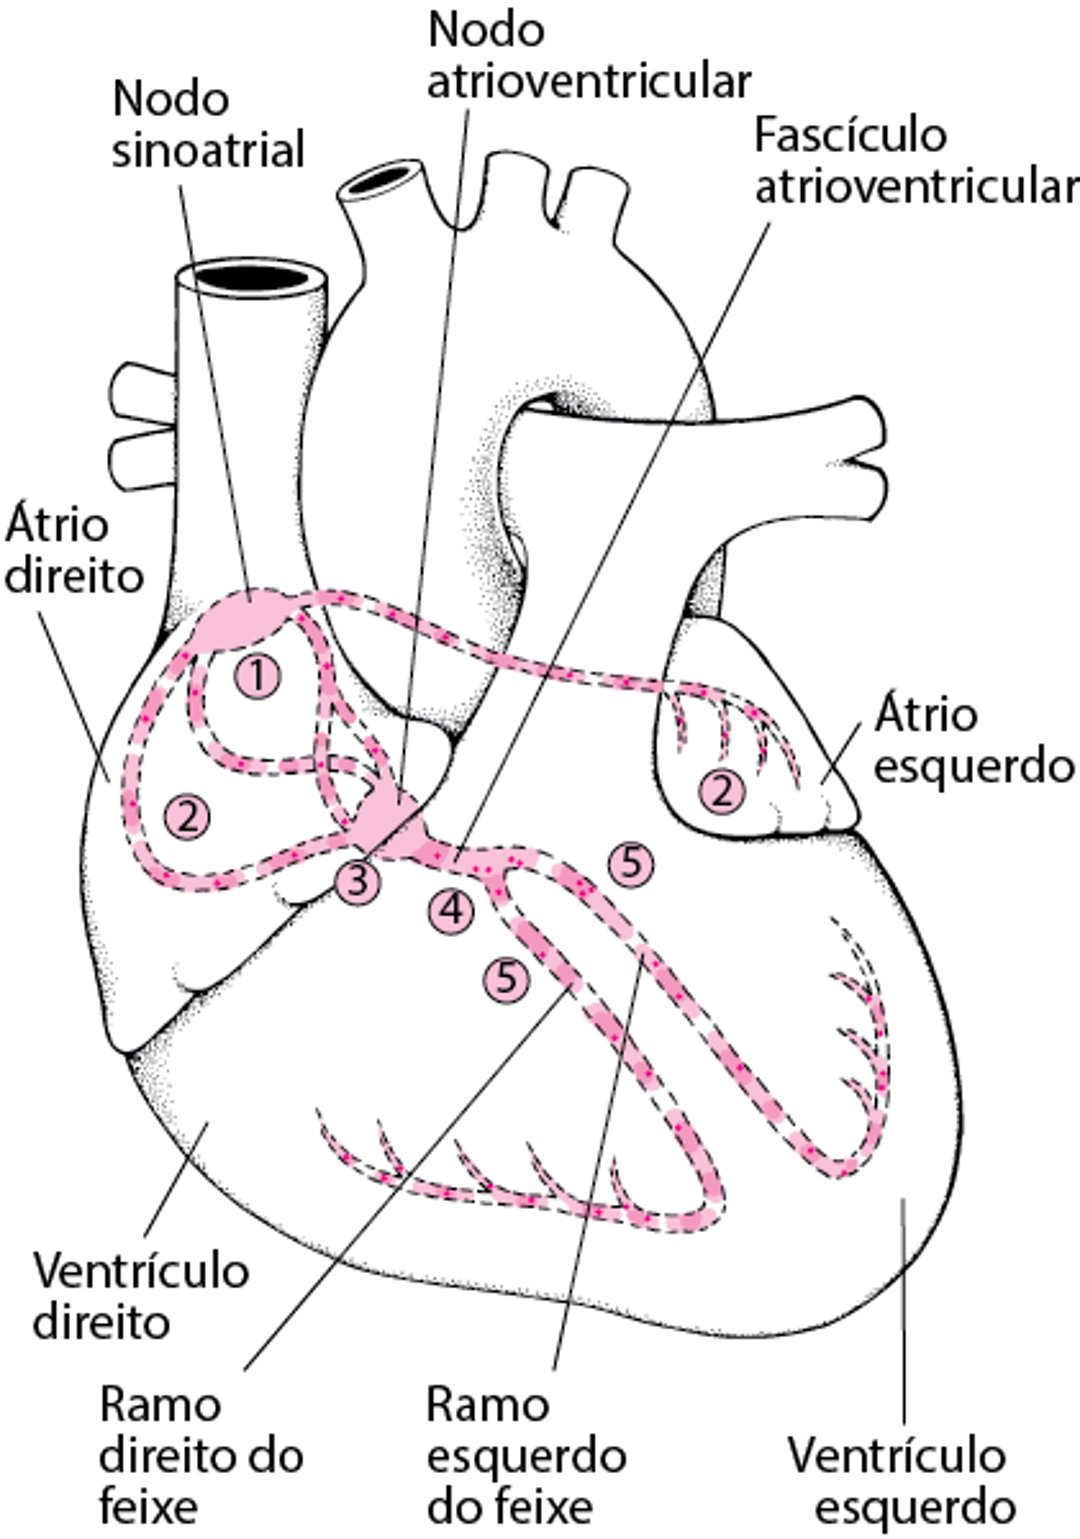
\includegraphics[width=0.6\textwidth]{figuras/coracao_sistema_eletrico.png} % insere o tikzpicture puro
  \label{fig:coracao_esquema_eletrico}
    \legend{Fonte: Adaptado de \citeonline{Mitchell_Arritmias_MSD}}
\end{figure}

Segundo \citeonline{Mitchell_Arritmias_MSD}, o batimento cardíaco normal se inicia no nódulo sinusal (1), localizado no átrio direito, que atua como o marcapasso natural do coração. A corrente elétrica propaga-se do átrio direito para o esquerdo (2), promovendo sua contração e o bombeamento do sangue para os ventrículos. Em seguida, o impulso atinge o nódulo atrioventricular (3) — conexão entre os átrios e ventrículos — onde é temporariamente retardado, permitindo que os átrios se contraiam completamente e encham as câmaras inferiores.

Posteriormente, a corrente percorre o feixe de His (4), que se divide e conduz o impulso para ambos os ventrículos (5), promovendo sua contração e o bombeamento do sangue para o restante do corpo.

\section{O eletrocardiograma}
\label{sec:ecg}

O eletrocardiograma, ECG, é um enxame não invasivo usado para medir a atividade elétrica do coração. Ele é feito a partir do contato de eletrodos, chamados de derivações ou \textit{leads}, sobre a pele.
A quantidade de eletrodos varia, mas geralmente são 12 \cite{msd_ecg}.

Ao registrar a magnitude e direção da corrente, as derivações geram uma onda que representa a atividade elétrica do coração. O passo a passo descrito em \ref{sec:funciionamento_coracao} é refletido em sua morfologia.

Na figura \ref{fig:ecg_exemplo_coracao}, um  ECG de um batimento, observe que ele é subdividido em: onda P, complexo QRS e onda T \cite{msd_ecg}. Note que cada uma dessas partes se refere a um estágio do batimento.

\begin{figure}[H]
  \centering
  \caption{Exemplo de ECG com sua morfologia destacada}
   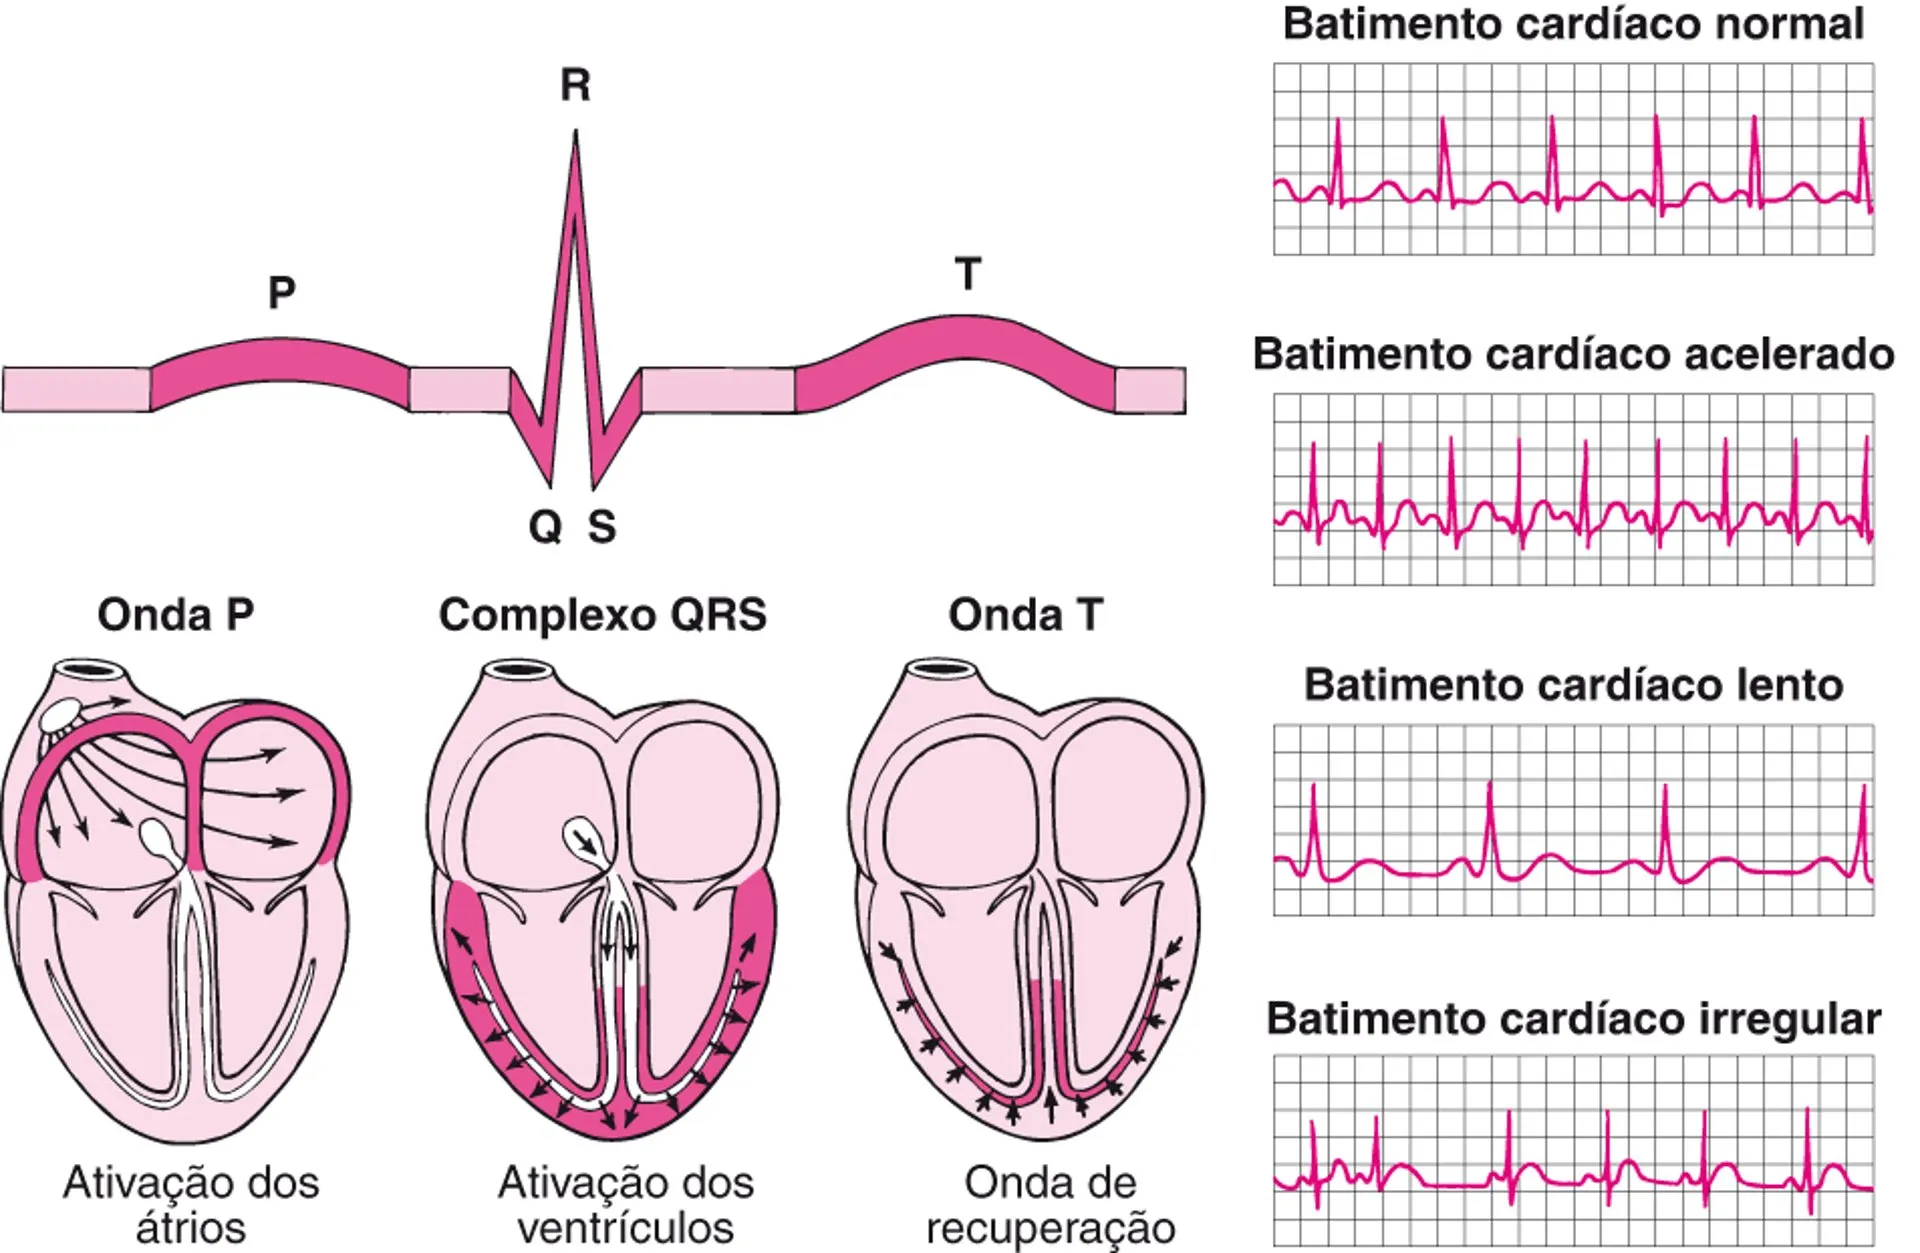
\includegraphics[width=0.8\textwidth]{figuras/ecg_exemplo_coracao.png} % insere o tikzpicture puro
  \label{fig:ecg_exemplo_coracao}
    \legend{Fonte: Adaptado de  \citeonline{msd_ecg}}
\end{figure}

Dentre as doenças que podem ser diagnósticas via ECG estão as arritmias cardíacas. 

\section{Arritmias}


\subsection{Arritmias clínicas}

As arritmias são alterações no ritmo cardíaco que podem ter diversas causas, incluindo alterações hormonais, uso de medicamentos, toxinas (como álcool ou cafeína), anomalias eletrolíticas ou doenças cardíacas.
Segundo \citeonline{Mitchell_Arritmias_MSD}, em adultos em repouso, a frequência cardíaca normal varia entre 60 e 100 batimentos por minuto (bpm). Frequências mais baixas, conhecidas como bradicardia sinusal, são comuns em atletas, crianças pequenas, adolescentes, jovens adultos e durante o sono. Por outro lado, a taquicardia sinusal ocorre quando a frequência se eleva, podendo ser observada durante o esforço físico, doenças, estimulação neural simpática ou emoção intensa.

Variações no ritmo cardíaco são fenômenos fisiológicos normais. Durante a respiração, por exemplo, é comum que a frequência aumente e diminua levemente — comportamento conhecido como arritmia sinusal respiratória. O autor ainda observa que um ritmo cardíaco perfeitamente regular pode indicar patologias no sistema nervoso autônomo, como ocorre em casos de diabetes avançado. Dessa forma, ainda não existe um indicador global e definitivo do que seria um ritmo sinusal considerado saudável.
As arritmias podem ser classificadas de forma simplificada em três tipos principais:

\begin{enumerate}
    \item Taquicardia: frequência excessivamente rápida;
    \item Bradicardia: frequência excessivamente lenta;
    \item Irregular: quando os impulsos percorrem o coração por vias irregulares.
\end{enumerate}

\subsection{Padrões de classificação para algoritmos (AAMI)}

A AAMI define cinco classes de arritmia: normal (N), ventricular (V), supraventricular (S), fusão (F) e não classificado (Q) \cite{silva2025,saadatnejad2020}.

As arritmias ventriculares incluem, por exemplo, as contrações prematuras ventriculares (PVCs) e os batimentos de escape. De acordo com \citeonline{Sattar_Premature_2025}, as PVCs são batimentos originários dos ventrículos que podem ocorrer mesmo em indivíduos saudáveis. Sua morfologia é variável, dependendo da origem do impulso, de doenças estruturais ou ainda de uso de medicamentos. Quando frequentes, podem causar fadiga e palpitações, evoluindo para disfunções ventriculares e, em alguns casos, representando a primeira manifestação de cardiopatias estruturais.

\citeonline{msdmanuals_ventricular} cita ainda outras causas potenciais de PVCs, como doenças da artéria coronária (especialmente durante ou após infarto), dilatação ventricular decorrente de insuficiência cardíaca e alterações nas válvulas cardíacas. Em pacientes com doenças estruturais, as PVCs podem progredir para arritmias mais graves, como taquicardia ventricular (VT) e fibrilação ventricular (FV), que representam risco de morte súbita.

\citeonline{mitchell2024afib,mitchell2024vt} descrevem tanto a fibrilação quanto a taquicardia ventricular como arritmias originadas nos ventrículos.
A fibrilação ventricular (FV) é caracterizada por batimentos rápidos e desordenados, resultantes de sinais elétricos caóticos nos ventrículos. Essa condição leva à perda de consciência em poucos segundos e à morte caso não haja intervenção imediata, configurando-se como um tipo de parada cardíaca. Entre suas causas estão afogamentos, choques elétricos e falha cardíaca.

A taquicardia ventricular (TV), por outro lado, produz uma frequência cardíaca de até 120 bpm e é formada por uma sequência de contrações ventriculares prematuras (PVCs). Quando persiste por mais de 30 segundos, recebe a denominação de taquicardia sustentada. Costuma ocorrer em indivíduos com alterações estruturais cardíacas, como infarto do miocárdio, falha cardíaca ou cardiomiopatia. Os sintomas incluem fraqueza, tontura e desconforto torácico. Caso persista por mais de 30 segundos, o tratamento é indicado mesmo na ausência de sintomas, uma vez que pode evoluir para fibrilação ventricular.

Apesar de ocorrerem também em indivíduos saudáveis, as PVCs possuem significância clínica, pois podem estar associadas a outros tipos de arritmias ventriculares graves. É importante considerar o contexto do batimento: no caso da taquicardia ventricular, por exemplo, o diagnóstico é estabelecido a partir de uma sequência de PVCs que produz uma frequência cardíaca elevada (>20 bpm). Assim, o diagnóstico depende de uma combinação de características temporais e morfológicas, observando-se o contexto dos batimentos e, naturalmente, os sintomas clínicos.

O batimento ventricular de escape, por sua vez, atua como um mecanismo compensatório, funcionando como um “backup” protetivo do coração quando o marcapasso natural falha temporariamente.

Dentro da classe dos batimentos normais, além do batimento típico descrito na \ref{sec:funciionamento_coracao}, incluem-se também os batimentos atriais de escape e os bloqueios do ramo esquerdo e direito. Estes últimos, embora inofensivos por si só, podem indicar condições cardíacas subjacentes mais graves, como doença da artéria coronária ou infarto do miocárdio prévio \cite{mitchell2024hisbloqueio}.

